%% Copernicus Publications Manuscript Preparation Template for LaTeX Submissions
%% ---------------------------------
%% This template should be used for copernicus.cls
%% The class file and some style files are bundled in the Copernicus Latex Package, which can be downloaded from the different journal webpages.
%% For further assistance please contact Copernicus Publications at: production@copernicus.org
%% https://publications.copernicus.org/for_authors/manuscript_preparation.html


%% Please use the following documentclass and journal abbreviations for preprints and final revised papers.

%% 2-column papers and preprints
\documentclass[amt, manuscript]{copernicus}



%% Journal abbreviations (please use the same for preprints and final revised papers)

%% \usepackage commands included in the copernicus.cls:
%\usepackage[german, english]{babel}
%\usepackage{tabularx}
%\usepackage{cancel}
%\usepackage{multirow}
%\usepackage{supertabular}
%\usepackage{algorithmic}
%\usepackage{algorithm}
%\usepackage{amsthm}
%\usepackage{float}
%\usepackage{subfig}
%\usepackage{rotating}


\begin{document}

\title{TEXT}


% \Author[affil]{given_name}{surname}

\Author[]{}{}
\Author[]{}{}
\Author[]{}{}

\affil[]{ADDRESS}
\affil[]{ADDRESS}

%% The [] brackets identify the author with the corresponding affiliation. 1, 2, 3, etc. should be inserted.

%% If an author is deceased, please mark the respective author name(s) with a dagger, e.g. "\Author[2,$\dag$]{Anton}{Aman}", and add a further "\affil[$\dag$]{deceased, 1 July 2019}".

%% If authors contributed equally, please mark the respective author names with an asterisk, e.g. "\Author[2,*]{Anton}{Aman}" and "\Author[3,*]{Bradley}{Bman}" and add a further affiliation: "\affil[*]{These authors contributed equally to this work.}".


\correspondence{NAME (EMAIL)}

\runningtitle{TEXT}

\runningauthor{TEXT}



\firstpage{1}

\maketitle



\begin{abstract}
TEXT
\end{abstract}


\copyrightstatement{TEXT}


\introduction  %% \introduction[modified heading if necessary]
TEXT
\section{Introduction}

\section{Data and methods}
\subsection{Ice Cloud Imager}


\subsection{ICI simulations}
%
The satellite observations for all ICI channels are simulated with the Atmospheric Radiative Transfer Simulator (ARTS).   

\subsection{QRNN}

%
The neural network training is a process of learning to predict the outputs {$y_i$} from inputs {$x_i$} through a series of learnable transformations. While training, neural networks seek to minimise the model error through a loss function. The choice of the loss function depends on the predictive problem. When a neural network is trained to minimise the mean of the quantile loss function to predict the quantiles of the distribution, it is called a Quantile Regression Neural Network (QRNN). 



\subsection{Training data}

Out of the 125\,000 simulations, 100\,000 are selected to form the training data. The remaining are used for testing. In the training data, 90\% of the data is randomly selected to form the training data, while the other 10\% form the \textit{testing-during-training} database. 

The training sample combines measurements from all 183 GHz channels and the available sub-millimeter channels. For ICI, the training set combines data from 183\,GHz, 325 GHz, 448\,GHz and 664\,GHz to predict cloud corrected observations for the target 183 GHz. For each 183 GHz channel, QRNN needs to be trained separately with a new target value. 

ARTS simulations are noise free, so to incorporate the satellite measurement uncertainties, gaussian noise is added to the input training data according to the channel NE$\Delta$T. The target training data is kept noise free. In order to build a robust learning network, random noise is added to the inputs at each training iteration. This exposes the model to a different datasets during the entire training process and avoids the memorisation of training samples. The input data is also normalized with mean and standard deviation.

\subsection{QRNN model selection}

A high performing QRNN model requires tuning of multiple hyperparameters. These parameters determine the structure and the training set-up of the neural network. Several of these hyper-parameters are non-learnable, and must be defined before beginning the training.

Among the structural parameters, a grid search was performed to determine the number of neurons (width) and hidden layers(depth). The quantile loss and CRPS on the validation set averaged over all predicted quantiles is used to compare the performance of different hyper-parameter configurations. 

We did not optimise the type of activation function and batch size. Rectified Linear Unit (ReLU) was used as the activation function  and the batch size was set to 128 samples for all QRNN models. 

The training process is optimized through different training parameters e.g. batch size, learning rate, number of epochs, momentum, decay. A customised  learning rate scheduler has been implemented to optimise SGD. The initial learning rate was revised after a certain number of epochs.  We started the training process with a initial learning rate of 0.1, and decreased it by a factor of 10 after 100 epochs. The best neural network performance was obtained when the network was trained three times with a new initial learning rate. For each training  if the validation loss remained unchanged till 6 training epochs, the learning rate was reduced by a factor of 2. 

\begin{figure}[p]
	\centering
	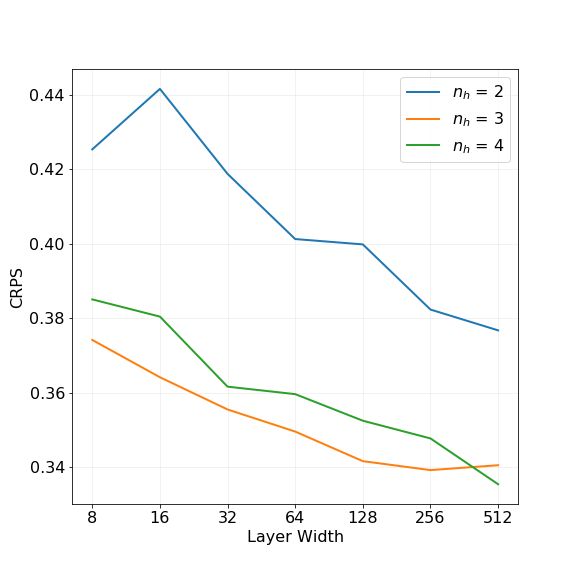
\includegraphics[height=57mm]{Figures/CRPS.png} 
	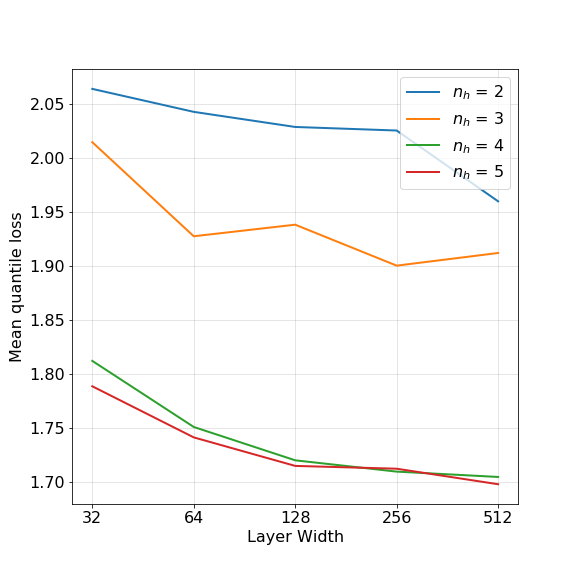
\includegraphics[height=57mm]{Figures/quantile_loss.png}
	\caption{}
	\label{fig:}	
\end{figure}

\section{Results}
\subsection{Prediction results}

The prediction output from QRNN is in form of quantiles $x_{\tau}$, for median, $\pm 1\sigma$, $\pm 2 \sigma$ and  $\pm 3 \sigma$ ($\tau$ = 0.002, 0.03, 0.16, 0.5, 0.84, 0.97, 0.998). The expectation value of the posterior distribution is assumed to be the best estimate for the predicted clear-sky value.  

\begin{figure}[p]
	\centering
	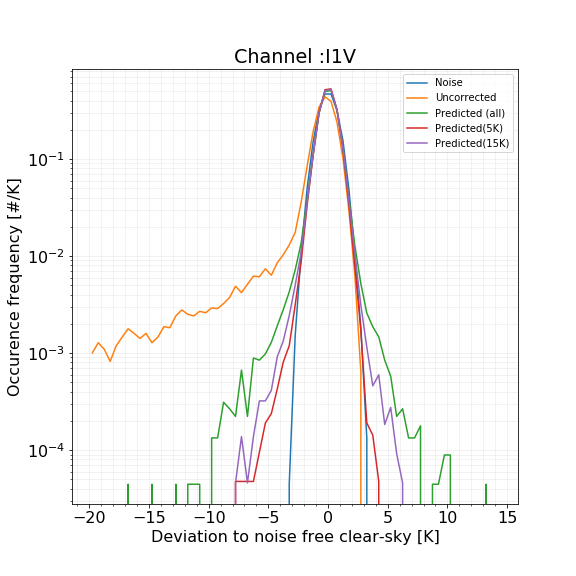
\includegraphics[height=57mm]{Figures/ICI_I1V.png} 
	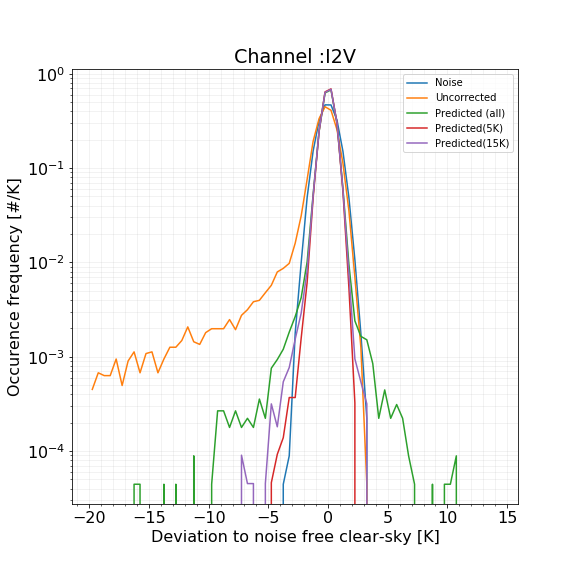
\includegraphics[height=57mm]{Figures/ICI_I2V.png}
	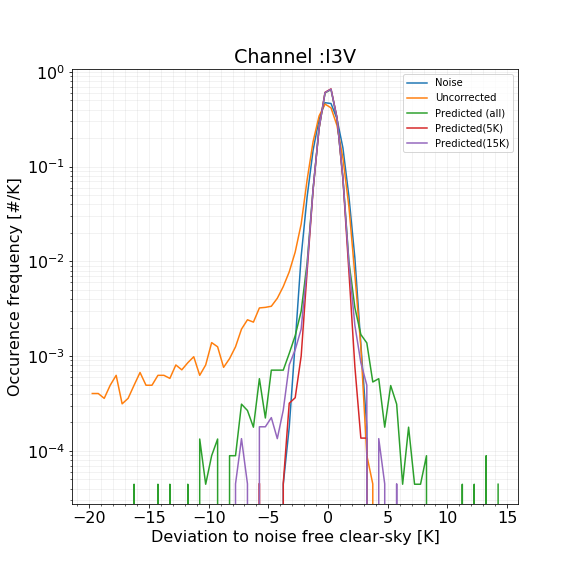
\includegraphics[height=57mm]{Figures/ICI_I3V.png} 
	\caption{}
	\label{fig:}	
\end{figure}

\begin{table}[!p]
	\centering
	\begin{tabular}{lrrrr}
		\hline
		Dataset              &   bias &   std &   measure skewness &   rejected \\
		\hline
		Noise                &   0.00 &  0.80 &              -0.00 &       - \\
		uncorrected          &  -1.59 &  7.78 &              -8.88 &       - \\
		corrected (all)      &  -0.08 &  1.14 &               0.52 &       - \\
		corrected (filtered) &  -0.13 &  0.98 &              -0.34 &       5.50 \\
		\hline
	\end{tabular}
	\caption{I1V}
\end{table}

\begin{table}[!p]
	\centering
	\begin{tabular}{lrrrr}
		\hline
		Dataset              &   bias &   std &   measure skewness &   rejected \\
		\hline
		Noise                &  -0.01 &  0.80 &               0.02 &       - \\
		uncorrected          &   7.37 &  8.15 &              -7.80 &       - \\
		corrected (all)      &  -0.09 &  0.79 &               0.85 &       - \\
		corrected (filtered) &  -0.12 &  0.65 &               0.12 &       3.02 \\
		\hline
	\end{tabular}
	\caption{I2V}
\end{table}

\begin{table}[!p]
	\centering
	\begin{tabular}{lrrrr}
		\hline
		Dataset              &   bias &   std &   measure skewness &   rejected \\
		\hline
		Noise                &  0.00 & 0.80 &             -0.02 &      - \\
		uncorrected          & 14.64 & 8.66 &             -6.67 &      - \\
		corrected (all)      & -0.10 & 0.76 &              0.45 &      - \\
		corrected (filtered) & -0.11 & 0.64 &              0.20 &      1.57 \\
		\hline
	\end{tabular}
	\caption{I3V}
\end{table}

\begin{figure}[p]
	\centering
	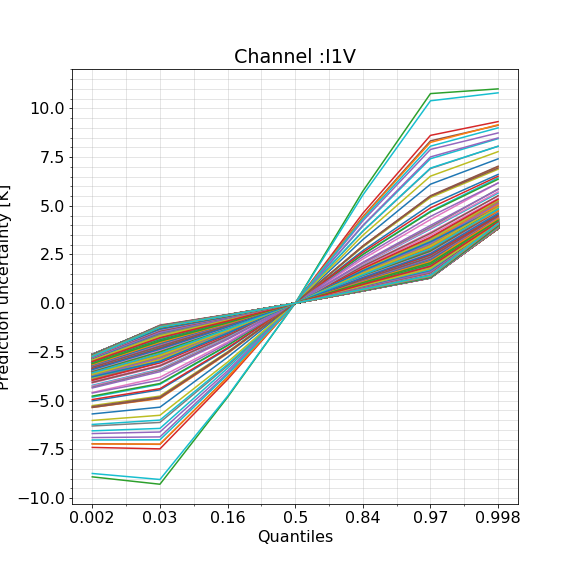
\includegraphics[height=57mm]{Figures/prediction_uncertainty_I1V.png} 
	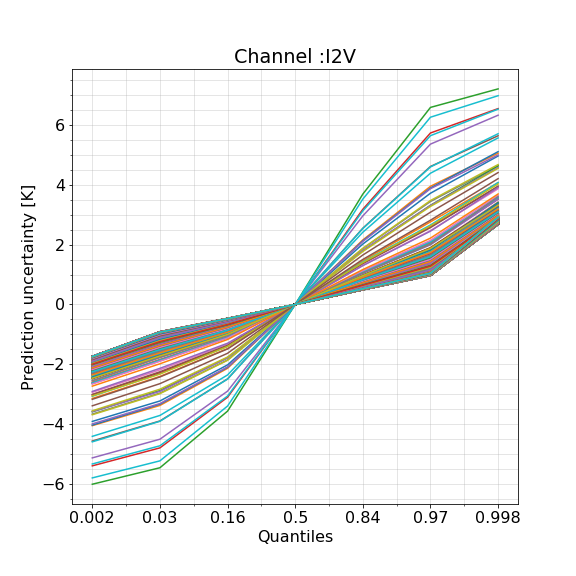
\includegraphics[height=57mm]{Figures/prediction_uncertainty_I2V.png}
	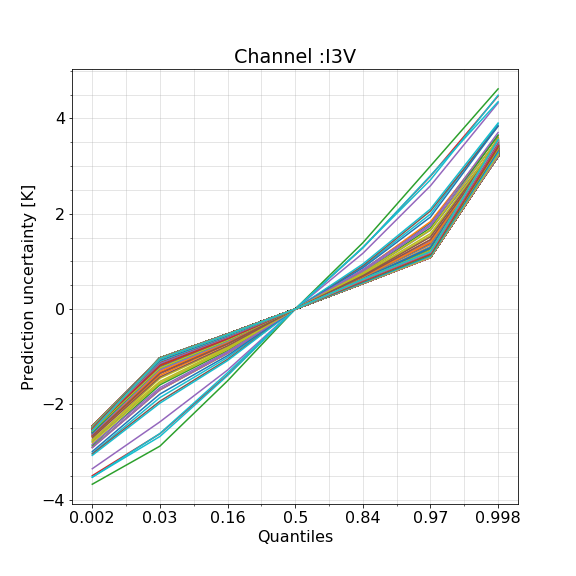
\includegraphics[height=57mm]{Figures/prediction_uncertainty_I3V.png} 
	\caption{}
	\label{fig:}	
\end{figure}
\subsection{Uncertainty quantification}


\section{Special case of using only 325\,GHz for cloud correction}

\subsection{Data}
24 monochromatic frequencies were used so that each channel could be represented
with sufficient accuracy. The simulations were generated for sensor viewing angles from
$0^{\circ}$ to $45^{\circ}$, but all the results described here are based on nadir viewing angle.


\subsection{Training}

\subsection{Prediction results}


\conclusions  %% \conclusions[modified heading if necessary]


%% The following commands are for the statements about the availability of data sets and/or software code corresponding to the manuscript.
%% It is strongly recommended to make use of these sections in case data sets and/or software code have been part of your research the article is based on.

\codeavailability{TEXT} %% use this section when having only software code available


\dataavailability{TEXT} %% use this section when having only data sets available


\codedataavailability{TEXT} %% use this section when having data sets and software code available


\sampleavailability{TEXT} %% use this section when having geoscientific samples available


\videosupplement{TEXT} %% use this section when having video supplements available


\appendix
\section{}    %% Appendix A

\subsection{}     %% Appendix A1, A2, etc.


\noappendix       %% use this to mark the end of the appendix section. Otherwise the figures might be numbered incorrectly (e.g. 10 instead of 1).

%% Regarding figures and tables in appendices, the following two options are possible depending on your general handling of figures and tables in the manuscript environment:

%% Option 1: If you sorted all figures and tables into the sections of the text, please also sort the appendix figures and appendix tables into the respective appendix sections.
%% They will be correctly named automatically.

%% Option 2: If you put all figures after the reference list, please insert appendix tables and figures after the normal tables and figures.
%% To rename them correctly to A1, A2, etc., please add the following commands in front of them:

\appendixfigures  %% needs to be added in front of appendix figures

\appendixtables   %% needs to be added in front of appendix tables

%% Please add \clearpage between each table and/or figure. Further guidelines on figures and tables can be found below.



\authorcontribution{TEXT} %% this section is mandatory

\competinginterests{TEXT} %% this section is mandatory even if you declare that no competing interests are present

\disclaimer{TEXT} %% optional section

\begin{acknowledgements}
TEXT
\end{acknowledgements}




%% REFERENCES


 \bibliographystyle{copernicus}
 \bibliography{example.bib}

\end{document}
